\documentclass[border=10pt]{standalone}
\usepackage{amsmath}
\usepackage{amssymb}
\usepackage{tikz}
\usetikzlibrary{arrows.meta,calc,decorations.pathreplacing,patterns,shapes.geometric,positioning,shadings,decorations.markings,decorations.pathmorphing}

\begin{document}
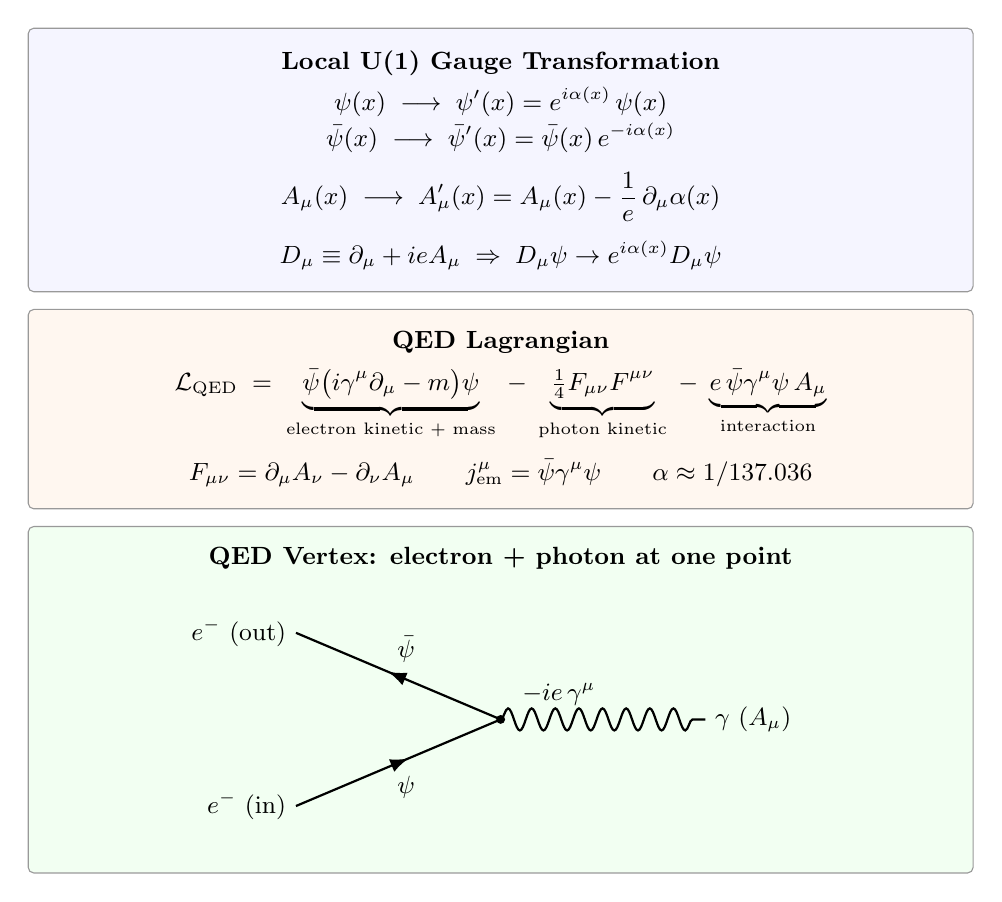
\begin{tikzpicture}[
  font=\small,
  >=Latex,
  panel/.style={draw=black!40, rounded corners=2pt, fill=#1, inner sep=8pt},
  electron/.style={postaction={decorate}, decoration={markings,
    mark=at position 0.55 with {\arrow{Latex}}}},
  photon/.style={decorate, decoration={snake, amplitude=1.4mm, segment length=3mm, post length=1mm}}
]

% =========================================================
% TOP PANEL: Local U(1) Gauge Transformation
% =========================================================
\node[panel=blue!4, minimum width=12cm, anchor=north] (top) at (0,0) {
  \begin{minipage}{11.4cm}
    \centering
    \textbf{Local U(1) Gauge Transformation}\\[4pt]
    $\psi(x)\;\longrightarrow\;\psi'(x) = e^{i\alpha(x)}\,\psi(x)$\\[2pt]
    $\bar\psi(x)\;\longrightarrow\;\bar\psi'(x) = \bar\psi(x)\,e^{-i\alpha(x)}$\\[6pt]
    $A_\mu(x)\;\longrightarrow\;A'_\mu(x) = A_\mu(x) - \dfrac{1}{e}\,\partial_\mu\alpha(x)$\\[6pt]
    $D_\mu \equiv \partial_\mu + i e A_\mu \;\Rightarrow\; D_\mu\psi \to e^{i\alpha(x)} D_\mu\psi$
  \end{minipage}
};

% =========================================================
% MIDDLE PANEL: QED Lagrangian
% =========================================================
\node[panel=orange!6, minimum width=12cm, anchor=north, yshift=-6pt] (mid) at (top.south) {
  \begin{minipage}{11.4cm}
    \centering
    \textbf{QED Lagrangian}\\[4pt]
    $\displaystyle \mathcal{L}_{\mathrm{QED}} \;=\; \underbrace{\bar\psi\bigl(i\gamma^\mu\partial_\mu - m\bigr)\psi}_{\text{electron kinetic + mass}}
    \;-\;\underbrace{\tfrac{1}{4} F_{\mu\nu}F^{\mu\nu}}_{\text{photon kinetic}}
    \;-\;\underbrace{e\,\bar\psi\gamma^\mu\psi\,A_\mu}_{\text{interaction}}$\\[6pt]
    $F_{\mu\nu} = \partial_\mu A_\nu - \partial_\nu A_\mu \qquad
     j^\mu_{\mathrm{em}} = \bar\psi\gamma^\mu\psi \qquad
     \alpha \approx 1/137.036$
  \end{minipage}
};

% =========================================================
% BOTTOM PANEL: QED vertex Feynman diagram
% =========================================================
\node[panel=green!5, minimum width=12cm, minimum height=4.4cm, anchor=north, yshift=-6pt] (bot) at (mid.south) {};
\node[anchor=north] at ($(bot.north)+(0,-0.15)$) {\textbf{QED Vertex: electron + photon at one point}};

% Geometry: vertex at origin of local coordinates inside the panel
\begin{scope}[shift={($(bot.center)+(0,-0.25)$)}]
  % vertex point
  \coordinate (V) at (0,0);
  % electron in (lower-left)
  \coordinate (Ein) at (-2.6,-1.1);
  % electron out (upper-left)
  \coordinate (Eout) at (-2.6, 1.1);
  % photon (right)
  \coordinate (P) at (2.6, 0);

  % electron lines with arrows
  \draw[electron, thick] (Ein) -- (V);
  \draw[electron, thick] (V) -- (Eout);

  % photon (wavy)
  \draw[photon, thick] (V) -- (P);

  % vertex blob
  \fill[black] (V) circle (1.6pt);

  % Labels
  \node[anchor=east] at (Ein) {$e^-$ (in)};
  \node[anchor=east] at (Eout) {$e^-$ (out)};
  \node[anchor=west] at (P) {$\gamma$ ($A_\mu$)};

  % Coupling label near vertex
  \node[anchor=south west] at ($(V)+(0.15,0.05)$) {$-i e\,\gamma^\mu$};

  % small annotations
  \node[anchor=north] at ($(Ein)!0.5!(V)+(0.1,-0.05)$) {$\psi$};
  \node[anchor=south] at ($(V)!0.5!(Eout)+(0.1,0.05)$) {$\bar\psi$};
\end{scope}

\end{tikzpicture}
\end{document}
